% This file contains the content for a main section
\regularsectionformat	% Change formatting to that of a main, numbered section
%% Modify below this line %%

% Define a local macro - FieldName, description, comment
\newcommand{\xmlfield}[3]{
	\TabPositions{2em,1.75in,2.5in,2.6in}
	\tab\texttt{#1} \tab#2 \tab// #3	 \par
}

\chapter{Data Model}

This section describes the data intended for use within the ACES Metadata file.

All top level structures shall be tagged as being within the \texttt{aces} namespace with urn \\ \texttt{urn:acesMetadata:acesMetadataFile:v1.0}

\section{UML Diagram}
The following UML diagrams are segments of the complete UML diagram which is not included in this document due to space constraints.  To view the entire UML diagram in SVG format visit \url{https://aces.mp/amf\_uml}.

\subsection{acesMetadataFile}
\begin{figure}[H]
  \centering
  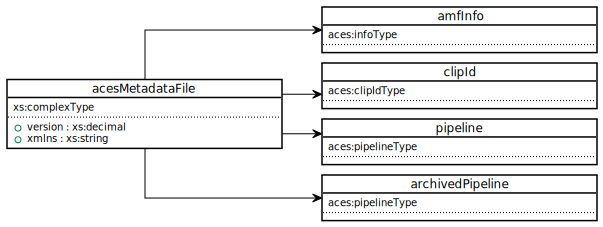
\includegraphics[width=0.66\textwidth]{./uml_diagrams/uml_amf.pdf}
\end{figure}

\subsection{amfInfo}
\begin{figure}[H]
  \centering
  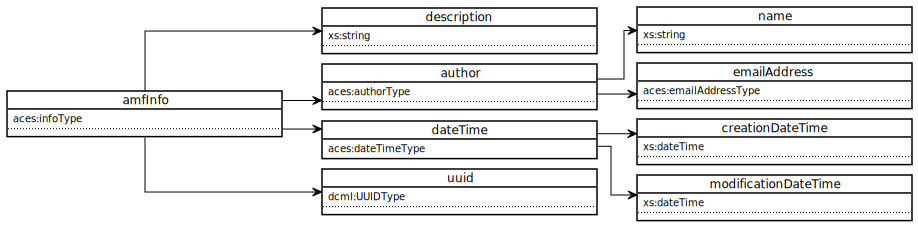
\includegraphics[width=\textwidth]{./uml_diagrams/uml_amfInfo.pdf}
\end{figure}

\subsection{clipId}
\begin{figure}[H]
  \centering
  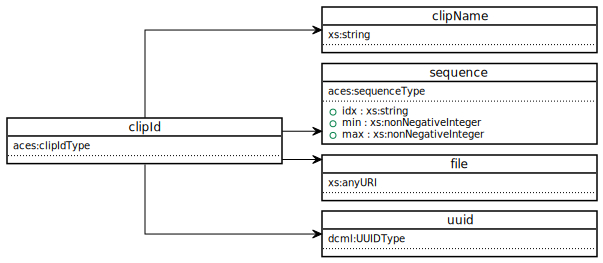
\includegraphics[width=0.75\textwidth]{./uml_diagrams/uml_clipId.pdf}
\end{figure}

\subsection{pipeline}
\begin{figure}[H]
  \centering
  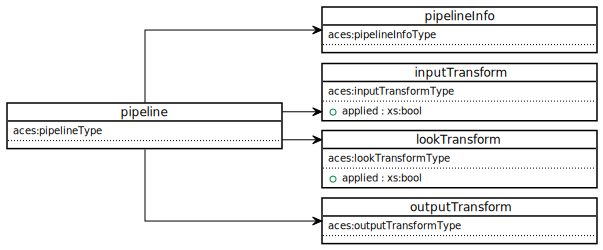
\includegraphics[width=0.66\textwidth]{./uml_diagrams/uml_pipeline.pdf}
\end{figure}

\subsection{pipelineInfo}
\begin{figure}[H]
  \centering
  \includegraphics[width=\textwidth]{./uml_diagrams/uml_pipelineInfo.pdf}
\end{figure}

\subsection{inputTransform}
\begin{figure}[H]
  \centering
  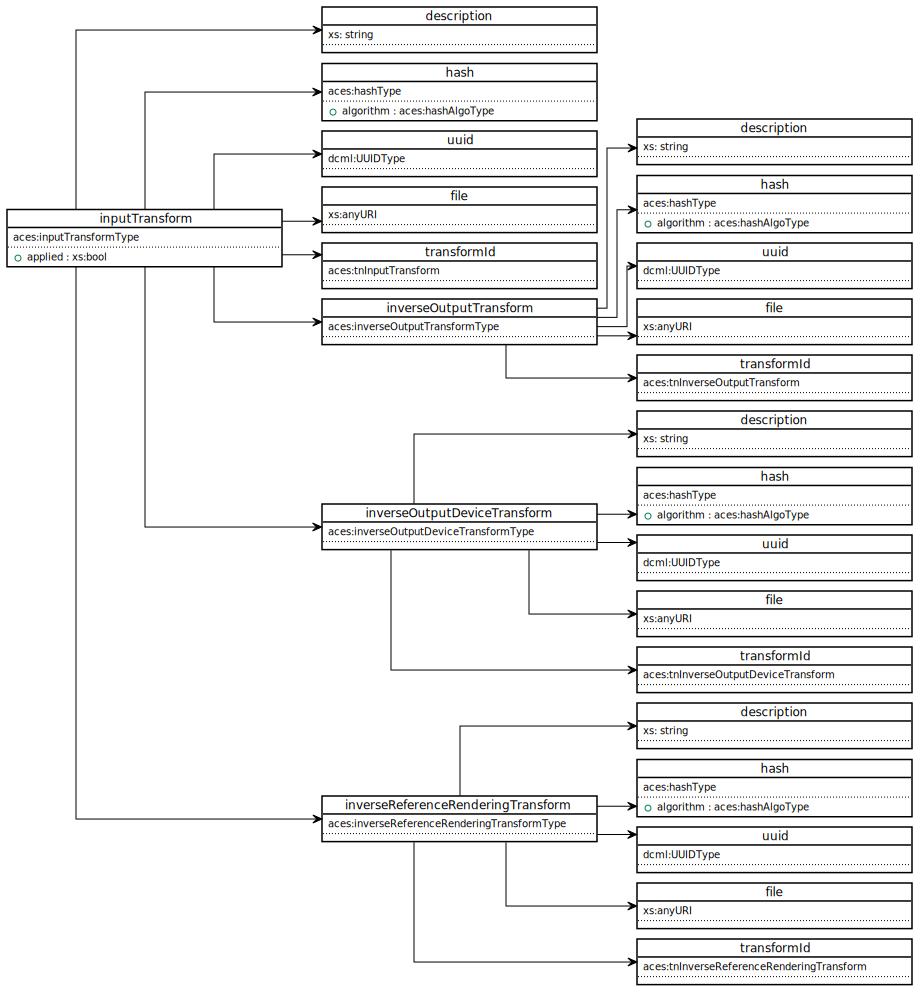
\includegraphics[width=\textwidth]{./uml_diagrams/uml_inputTransform.pdf}
\end{figure}

\subsection{lookTransform}
\begin{figure}[H]
  \centering
  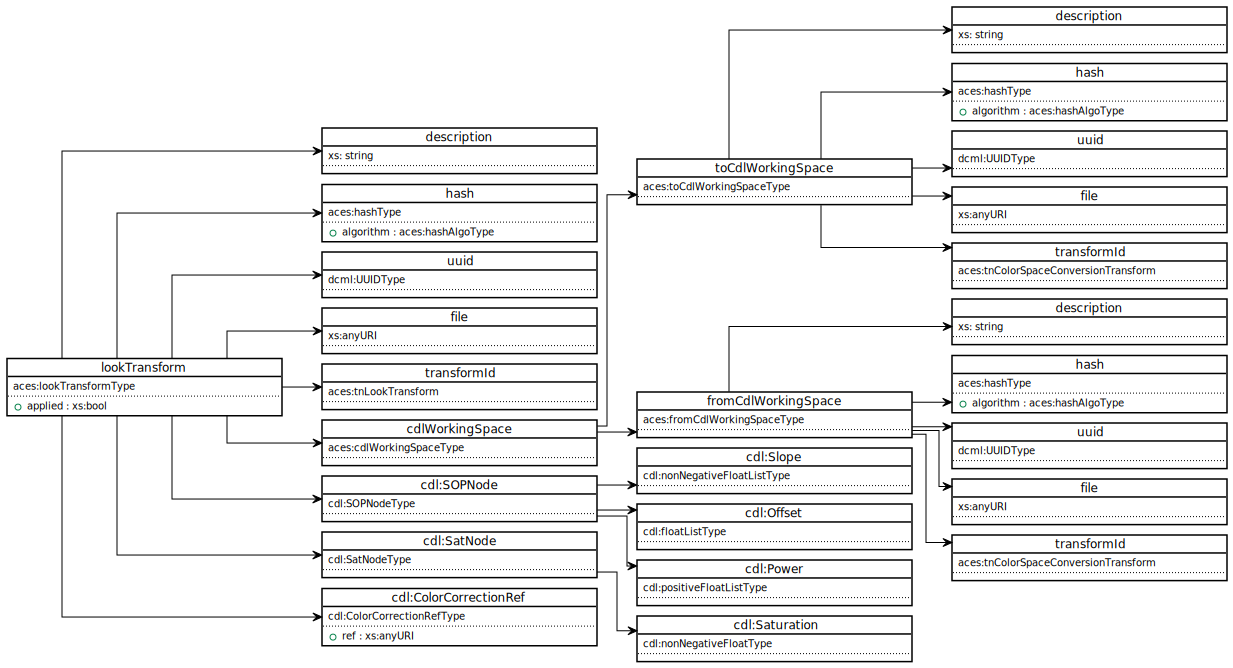
\includegraphics[width=\textwidth]{./uml_diagrams/uml_lookTransform.pdf}
\end{figure}

\subsection{outputTransform}
\begin{figure}[H]
  \centering
  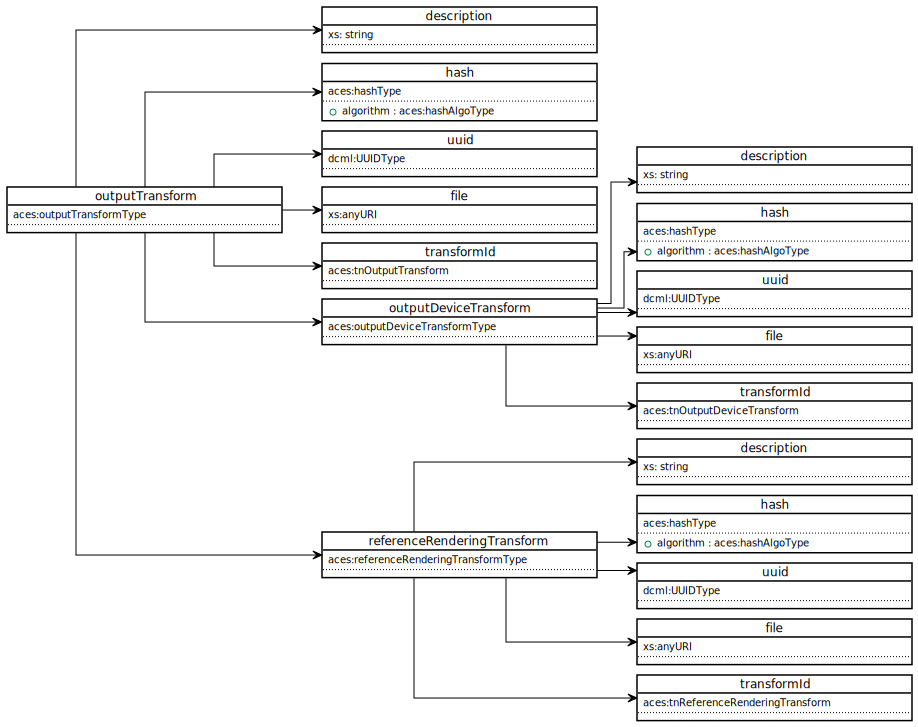
\includegraphics[width=\textwidth]{./uml_diagrams/uml_outputTransform.pdf}
\end{figure}


\section{Types}

The following types are defined for use within the AMF XML file and are validated with the XSD schema included in Appendix A.  The types are used as the basis to form the elements listed in section X in the schema.

\input{sec-types.tex}


\newpage
\section{Elements (by type)}
%\settocdepth{section}

The following elements are defined for use with the AMF XML file and are validated with the XSD schema included in Appendix A. 

\newcommand\element[9]{
    \def\tempa{#1}%
    \def\tempb{#2}%
    \def\tempc{#3}%
    \def\tempd{#4}%
    \def\tempe{#5}%
    \def\tempf{#6}%
    \def\tempg{#7}%
    \def\temph{#8}%
    \def\tempi{#9}%
    \elementcontinued
}


\newcommand\elementcontinued[3]{
    \subsubsection{\textbf{ {\texttt{\tempa}} }}

    \textbf{Description:}
    \begin{adjustwidth}{5mm}{} \vspace{-1.5mm}
        \tempb
    \end{adjustwidth}

    \textbf{Diagram:}
    \begin{figure}[H]
        \includegraphics[width=3.5in]{\tempc}
    \end{figure}

    \textbf{Type:}
    \begin{adjustwidth}{5mm}{} \vspace{-1.5mm}
        \texttt{\tempd}
    \end{adjustwidth}

    \textbf{Required or Optional:}
    \begin{adjustwidth}{5mm}{} \vspace{-1.5mm}
        \tempe
    \end{adjustwidth}

    \textbf{Occurrences:}
    \begin{adjustwidth}{5mm}{} \vspace{-1.5mm}
        Min: \tempf~Max: \tempg
    \end{adjustwidth}

    \textbf{Attributes:}
    \begin{adjustwidth}{5mm}{} \vspace{-1.5mm}
        Required: \texttt{\temph} \\
        Optional: \texttt{\tempi}
    \end{adjustwidth}

    \textbf{Parent:}
    \begin{adjustwidth}{5mm}{} \vspace{-1.5mm}
        #1
    \end{adjustwidth}

    \textbf{Children:}
    \begin{adjustwidth}{5mm}{} \vspace{-1.5mm}
        #2
    \end{adjustwidth}

    \textbf{Example:}
    \begin{adjustwidth}{5mm}{} \vspace{-1.5mm}
        #3
    \end{adjustwidth}
}

\subsection{\texttt{aces:acesMetadataFile}}

\element{aces:acesMetadataFile}
        {The top level element of an ACES Metadata File.  This element defines first level child elements.}
        {images/acesMetadataFile_xsd_Element_aces_acesMetadataFile.png}
        {xs:element}
        {Required}
        {1}{1}
        {\texttt{version="1.0", xmlns:aces="urn:ampas:aces:amf:v1.0"}}{\texttt{xmlns, xsi:schemeLocation}}
        {None}
        {\texttt{aces:amfInfo, aces:archivedPipeline, aces:clipId, aces:pipeline}}
        { \lstinline{<aces:acesMetadataFile} \\
        \lstinline{xmlns:aces="urn:ampas:aces:amf:v1.0"} \\
        \lstinline{xsi:schemaLocation="urn:ampas:aces:amf:v1.0 file:acesMetadataFile.xsd"} \\ \lstinline{xmlns:cdl="urn:ASC:CDL:v1.01"}\\
        \lstinline{xmlns:xsi="http://www.w3.org/2001/XMLSchema-instance"}\\
        \lstinline{version="1.0">}\\
        ... \\
        \lstinline{</aces:acesMetadataFile>}}

\element{aces:acesMetadataFile / aces:amfInfo}
        {This element contains all the elements containing information about the AMF itself including author elements, date and time elements, a description element, and a UUID element.}
        {images/acesMetadataFile_xsd_Element_aces_amfInfo.png}
        {aces:infoType}
        {Required}
        {1}{1}
        {none}{none}
        {\texttt{aces:acesMetadataFile}}
        {\texttt{aces:author, aces:dateTime, aces:description, aces:uuid}}
        {\lstinline{<aces:amfInfo>} \\
        ... \\
        \lstinline{</aces:amfInfo>}}

\element{aces:acesMetadataFile / aces:archivedPipeline}
        {This element contains all the elements describing an ACES viewing pipeline archived for historical purposes.}
        {images/acesMetadataFile_xsd_Element_aces_archivedPipeline.png}
        {aces:pipelineType}
        {Optional}
        {0}
        {unbounded}
        {none}{none}
        {\texttt{aces:acesMetadataFile}}
        {\texttt{aces:inputTransform, aces:lookTransform, aces:outputTransform, aces:pipelineInfo}}
        {\lstinline{<aces:archivedPipeline>} \\
        ... \\
        \lstinline{</aces:archivedPipeline>}}

\element{aces:acesMetadataFile / aces:clipId}
        {This optional element contains all the elements describing the location of the media files associated with the AMF.}
        {images/acesMetadataFile_xsd_Element_aces_clipId.png}
        {aces:clipIdType}
        {Optional}{0}{1}
        {none}{none}{\texttt{aces:acesMetadataFile}}
        {\texttt{aces:clipName, aces:file, aces:sequence, aces:uuid}}
        {\lstinline{<aces:clipId>} \\
        ... \\
        \lstinline{</aces:clipId>}}

\element{aces:acesMetadataFile / aces:pipeline}
        {This element contains all the elements describing the ACES viewing pipeline.}
        {images/acesMetadataFile_xsd_Element_aces_pipeline.png}
        {aces:pipelineType}
        {Required}{1}{1}
        {none}{none}
        {\texttt{aces:acesMetadataFile}}
        {\texttt{aces:inputTransform, aces:lookTransform, aces:outputTransform,\\ aces:pipelineInfo}}
        {\lstinline{<aces:pipeline>} \\
        ... \\
        \lstinline{</aces:pipeline>}}

\subsection{\texttt{aces:authorType}}

\element{aces:authorType / aces:emailAddress}
        {This element used to communicate the AMF author's email address.}
        {images/acesMetadataFile_xsd_Element_aces_emailAddress.png}
        {aces:emailAddressType}
        {Required}{1}{1}
        {none}{none}
        {\texttt{aces:author}}
        {None}
        {\lstinline{<aces:emailAddress>joe@onset.com</aces:emailAddress>}}

\element{aces:authorType / aces:name}
        {This element is used to communicate the name of the AMF author.}
        {images/acesMetadataFile_xsd_Element_aces_name.png}
        {\texttt{xs:string}}
        {Required}{1}{1}
        {None}{None}{\texttt{aces:author}}{None}{\lstinline{<aces:name>Joe Onset</aces:name>}}

\subsection{\texttt{aces:cdlWorkingSpaceType}}

\element{aces:cdlWorkingSpaceType / aces:fromCdlWorkingSpace}
        {This element contains all the elements describing the ACES Color Space Conversion transform used to convert from the Look Transform working color space in which an ASC-CDL is applied to ACES 2065-1.}
        {images/acesMetadataFile_xsd_Element_aces_fromCdlWorkingSpace.png}
        {\texttt{aces:workingSpaceTransformType}}
        {Required}{1}{1}
        {None}{None}
        {\texttt{aces:cdlWorkingSpace}}
        {aces:description, aces:file, aces:hash, aces:transformId, aces:uuid}
        {\lstinline{<aces:fromCdlWorkingSpace>} \\
        ... \\
        \lstinline{</aces:fromCdlWorkingSpace>}}

\element{aces:cdlWorkingSpaceType / aces:toCdlWorkingSpace}
        {This element contains all the elements describing the ACES Color Space Conversion transform used to convert from ACES 2065-1 to the Look Transform working color space in which an ASC-CDL transform is applied.  This transform shall be included when the working color space for the ASC-CDL Transform is not a working color space described in one of the Color Space Conversion transform included in the ACES core transforms.  When the working color space for the ASC-CDL Transform is a working color space described in one of the Color Space Conversion transform included in the ACES core transforms, the \texttt{aces:toCdlWorkingSpace} is optional.}
        {images/acesMetadataFile_xsd_Element_aces_toCdlWorkingSpace.png}
        {\texttt{aces:workingSpaceTransformType}}
        {Optional}{0}{1}
        {None}{None}
        {\texttt{aces:cdlWorkingSpace}}
        {\texttt{aces:description, aces:file, aces:hash, aces:transformId, aces:uuid}}
        {\lstinline{<aces:toCdlWorkingSpace>} \\
        ... \\
        \lstinline{</aces:toCdlWorkingSpace>}}
        
\subsection{\texttt{aces:clipIdType}}

\element{clipIdType / aces:clipName}
        {This element is used to communicate the clip name associated with the media files.}
        {images/acesMetadataFile_xsd_Element_aces_clipName.png}
        {\texttt{xs:string}}
        {Required}{1}{1}
        {None}{None}{\texttt{aces:clipId}}{None}{\lstinline{<aces:clipName>A001C012</aces:clipId>}}

\element{aces:clipIdType / aces:file}
        {This element is used to communicate the name of the media file.  Care should be taken when using the file name as an identifier as file locations and names typically change during production and post-production.}
        {images/acesMetadataFile_xsd_Element_aces_file.png}
        {\texttt{xs:anyURI}}
        {Choice of \texttt{aces:file}, \texttt{aces:sequence} or \texttt{aces:uuid} is required}{1}{1}
        {None}{None}{\texttt{aces:clipId}}{None}
        {\lstinline{<aces:file>file:///foo.mxf</aces:file>}}

\element{aces:clipIdType / aces:sequence}
        {This element is used to communicate the file sequence information associated with the media files.  The file sequence includes an index indicated by the \texttt{idx} attribute (e.g. \#) that is used to denote the location of frame numbers within the sequence string.  The \texttt{min} and \texttt{max} attributes are used to indicate the minimum frame number and maximum frame number of the sequence.  For example, if the sequence string is \texttt{movieFrame\#\#\#\#.exr} and attributes of \texttt{aces:sequence} are \texttt{idx='\#'}, \texttt{min='0'} and \texttt{min='1000'} the the media files associated with the AMF would be the frames numbered \texttt{movieFrame0000.exr} through \texttt{movieFrame1000.exr}}
        {images/acesMetadataFile_xsd_Element_aces_sequence.png}
        {\texttt{aces:sequenceType}}
        {Choice of \texttt{aces:file}, \texttt{aces:sequence} or \texttt{aces:uuid} is required}{1}{1}
        {\texttt{idx}, \texttt{min}, \texttt{max}}{None}{\texttt{aces:clipId}}{None}
        {\lstinline{<aces:sequence idx="#" min="1" max="240">A01_C012_AE0306_###.exr</aces:sequence>}}

\element{aces:clipIdType / aces:uuid}
		{This element is used to communicate a UUID associated with the media files referred to in the ClipID.}
		{images/acesMetadataFile_xsd_Element_aces_uuid.png}
		{\texttt{dcml:UUIDType}}
		{Choice of \texttt{aces:file}, \texttt{aces:sequence} or \texttt{aces:uuid} is required}{1}{1}
		{None}{None}
		{\texttt{aces:clipId}}{None}
		{\lstinline{<aces:uuid>urn:uuid:797c7cd8-4eb1-4f67-afce-af2b0a1d0285</aces:uuid>}}
		
\subsection{\texttt{aces:dateTimeType}}

\element{aces:dateTimeType / aces:creationDateTime}
		{This element is used to communicate the creation date and time of an AMF file or an ACES pipeline.}
		{images/acesMetadataFile_xsd_Element_aces_creationDateTime.png}
		{\texttt{xs:dateTime}}
		{Required}{1}{1}
		{None}{None}
		{\texttt{aces:dateTime}}{None}
		{\lstinline{<aces:creationDateTime>2020-11-10T13:20:00Z</aces:creationDateTime>}}

\element{aces:dateTimeType / aces:modificationDateTime}
		{This element is used to communicate the most recent modification date and time of an AMF file or an ACES pipeline.}
		{images/acesMetadataFile_xsd_Element_aces_modificationDateTime.png}
		{\texttt{xs:dateTime}}
		{Required}{1}{1}
		{None}{None}
		{\texttt{aces:dateTime}}{None}
		{\lstinline{<aces:modificationDateTime>2020-11-10T13:20:00Z</aces:modificationDateTime>}}
		
\subsection{\texttt{aces:infoType}}

\element{aces:infoType / aces:author}
		{This element contains all the elements describing the AMF author information.}
		{images/acesMetadataFile_xsd_Element_aces_author.png}
		{\texttt{xs:sequence}}
		{Optional}{1}{unbounded}
		{None}{None}
		{\texttt{aces:amfInfo}}{\texttt{aces:name, aces:emailAddress}}
		{\lstinline{<aces:author>} \\
        ... \\
        \lstinline{</aces:author>}}

\element{aces:infoType / aces:dateTime}
		{This element contains all the elements describing the date and time of the creation and modification of the AMF or an AMF pipeline.}
		{images/acesMetadataFile_xsd_Element_aces_dateTime.png}
		{\texttt{xs:sequence}}
		{Required}{1}{1}
		{None}{None}
		{\texttt{aces:amfInfo, aces:pipelineInfo}}{\texttt{aces:creationDateTime, modificationDateTime}}
		{\lstinline{<aces:dateTime>} \\
        ... \\
        \lstinline{</aces:dateTime>}}

\element{aces:infoType / aces:description}
		{This element is used to communicate description information for an AMF file or an ACES pipeline.}
		{images/acesMetadataFile_xsd_Element_aces_description.png}
		{\texttt{xs:string}}
		{Optional}{0}{1}
		{None}{None}
		{\texttt{aces:amfInfo, aces:piplineInfo}}{None}
		{\lstinline{<aces:description>Example movie</aces:description>}\\
		 \lstinline{<aces:description>Theatrical deliverable pipeline</aces:description>}}

\element{aces:infoType / aces:uuid}
		{This element is used to communicate a UUID associated with the AMF or an ACES pipeline.}
		{images/acesMetadataFile_xsd_Element_aces_uuid_10.png}
		{\texttt{dcml:UUIDType}}
		{Required}{0}{1}
		{None}{None}
		{\texttt{aces:amfInfo, aces:pipelineInfo}}{None}
		{\lstinline{<aces:uuid>urn:uuid:797c7cd8-4eb1-4f67-afce-af2b0a1d0285</aces:uuid>}}

\subsection{\texttt{aces:inputTransformType}}

\element{aces:inputTransformType / aces:file}
		{This element is used to communicate the location of a file used as an ACES Input Transform that transforms images encoded in a color space of a camera native file to ACES 2065-1.}
		{images/acesMetadataFile_xsd_Element_aces_file_1.png}
		{\texttt{xs:anyURI}}
		{Required}{0}{1}
		{None}{None}
		{\texttt{aces:inputTransform}}{None}
		{\lstinline{<aces:file>file:///inputTranforms.clf</aces:file>}}
		
\element{aces:inputTransformType / aces:inverseOutputDeviceTransform}
        {This element contains all the elements describing the transforms associated with an inverse output device transform used to convert output referred images to OCES.  This element is used in combination with \texttt{aces:inverseReferenceRenderingTransform} to convert output referred images to ACES 2065-1.}
        {images/acesMetadataFile_xsd_Element_aces_inverseOutputDeviceTransform.png}
        {\texttt{aces:inverseOutputTransformType}}
        {Required}{1}{1}
        {None}{None}
        {\texttt{aces:inputTransform}}
        {\texttt{aces:description, aces:file, aces:hash, aces:transformId, aces:uuid}}
        {\lstinline{<aces:inverseOutputDeviceTransform>} \\
        ... \\
        \lstinline{</aces:inverseOutputDeviceTransform>}}
        
\element{aces:inputTransformType / aces:inverseOutputTransform}
        {This element contains all the elements describing the transforms associated with an inverse output transform used to convert output referred images to ACES 2065-1.}
        {images/acesMetadataFile_xsd_Element_aces_inverseOutputTransform.png}
        {\texttt{aces:inverseOutputTransformType}}
        {Required}{1}{1}
        {None}{None}
        {\texttt{aces:inputTransform}}
        {\texttt{aces:description, aces:file, aces:hash, aces:transformId, aces:uuid}}
        {\lstinline{<aces:inverseOutputTransform>} \\
        ... \\
        \lstinline{</aces:inverseOutputTransform>}}
        
\element{aces:inputTransformType / aces:inverseReferenceRenderingTransform}
        {This element contains all the elements describing the transforms associated with an inverse reference rendering transform used to OCES images to ACES 2065-1.  This element is used in combination with texttt{aces:inverseOutputDeviceTransform} to convert output referred images to ACES 2065-1.}
        {images/acesMetadataFile_xsd_Element_aces_inverseReferenceRenderingTransform.png}
        {\texttt{aces:inverseReferenceRenderingTransformType}}
        {Required}{1}{1}
        {None}{None}
        {\texttt{aces:inputTransform}}
        {\texttt{aces:description, aces:file, aces:hash, aces:transformId, aces:uuid}}
        {\lstinline{<aces:inverseReferenceRenderingTransform>} \\
        ... \\
        \lstinline{</aces:inverseReferenceRenderingTransform>}}

\element{aces:inputTransformType / aces:transformId}
        {This element is used to communicate the transformID of an ACES Input Transform that transforms images encoded in a color space of a camera native file to ACES 2065-1.  For more information on transformIDs see S-2014-002 Academy Color Encoding System -- Versioning system.  Valid transforms for this element are Input Transforms.  The element is restricted to enforce the use of transformIDs that follow the IDT naming conventions established in the versioning system specification.  As noted in the versioning system specification, manufacturer and user created transforms shall be assigned a transformID according to patterns established in the document.}
        {images/acesMetadataFile_xsd_Element_aces_transformId.png}
        {\texttt{aces:tnInputTransform}}
        {Required}{1}{1}
        {None}{None}
        {\texttt{aces:inputTransform}}{None}
        {\lstinline{<aces:transformId>} \\
        \lstinline{urn:ampas:aces:transformId:v1.5:IDT.Sony.F65.a1.v1} \\
        \lstinline{</aces:transformId>}}
        
\element{aces:inputTransformType / aces:uuid}
		{This element is used to communicate the UUID of an ACES Input Transform that transforms images to ACES 2065-1.}
		{images/acesMetadataFile_xsd_Element_aces_uuid_1.png}
		{\texttt{dcml:UUIDType}}
		{Required}{0}{1}
		{None}{None}
		{\texttt{aces:inputTransform}}{None}
		{\lstinline{<aces:uuid>urn:uuid:797c7cd8-4eb1-4f67-afce-af2b0a1d0285</aces:uuid>}}
		

\subsection{\texttt{aces:inverseOutputDeviceTransformType}}
		
\element{aces:inverseOutputDeviceTransformType / aces:file}
		{This element is used to communicate the location of a file used as an ACES Inverse Output Device Transform that transforms images encoded in OCES color space to ACES 2065-1.}
		{images/acesMetadataFile_xsd_Element_aces_file_3.png}
		{\texttt{xs:anyURI}}
		{Required}{0}{1}
		{None}{None}
		{\texttt{aces:inputTransform}}{None}
		{\lstinline{<aces:file>file:///inverseOutputDeviceTransform.clf</aces:file>}}

\element{aces:inverseOutputDeviceTransformType / aces:transformId}
        {This element is used to communicate the transformID of an ACES Inverse Output Device Transform that transforms images encoded in an output referred color space to OCES.  For more information on transformIDs see S-2014-002 Academy Color Encoding System -- Versioning system.  Valid transforms for this element are Input Transforms.  The element is restricted to enforce the use of transformIDs that follow the InvODT naming conventions established in the versioning system specification.  As noted in the versioning system specification, manufacturer and user created transforms shall be assigned a transformID according to patterns established in the document.}
        {images/acesMetadataFile_xsd_Element_aces_transformId_2.png}
        {\texttt{aces:tnInverseDeviceOutputTransform}}
        {Required}{1}{1}
        {None}{None}
        {\texttt{aces:inputTransform}}{None}
        {\lstinline{<aces:transformId>} \\
        \lstinline{urn:ampas:aces:transformId:v1.5:InvODT.Academy.Rec709_100nits_dim.a1.0.3} \\
        \lstinline{</aces:transformId>}}

\element{aces:inverseOutputDeviceTransformType / aces:uuid}
		{This element is used to communicate the UUID of an ACES Inverse Output Device Transform that transforms images encoded in an output referred color space to OCES.}
		{images/acesMetadataFile_xsd_Element_aces_uuid_3.png}
		{\texttt{dcml:UUIDType}}
		{Required}{0}{1}
		{None}{None}
		{\texttt{aces:inputTransform}}{None}
		{\lstinline{<aces:uuid>urn:uuid:797c7cd8-4eb1-4f67-afce-af2b0a1d0285</aces:uuid>}}
\subsection{\texttt{aces:inverseOutputTransformType}}

\element{aces:inverseOutputTransformType / aces:file}
		{This element is used to communicate the location of a file used as an ACES Inverse Output Transform that transforms images encoded in an output referred color space to ACES.}
		{images/acesMetadataFile_xsd_Element_aces_file_2.png}
		{\texttt{xs:anyURI}}
		{Required}{0}{1}
		{None}{None}
		{\texttt{aces:inputTransform}}{None}
		{\lstinline{<aces:file>file:///inverseOutputTransform.clf</aces:file>}}

\element{aces:inverseOutputTransformType / aces:transformId}
        {This element is used to communicate the transformID of an ACES Inverse Output Transform that transforms images encoded in an output referred color space to ACES 2065-1.  For more information on transformIDs see S-2014-002 Academy Color Encoding System -- Versioning system.  Valid transforms for this element are Input Transforms.  The element is restricted to enforce the use of transformIDs that follow the InvRRTODT naming conventions established in the versioning system specification.  As noted in the versioning system specification, manufacturer and user created transforms shall be assigned a transformID according to patterns established in the document.}
        {images/acesMetadataFile_xsd_Element_aces_transformId_1.png}
        {\texttt{aces:tnInverseReferenceRenderingTransform}}
        {Required}{1}{1}
        {None}{None}
        {\texttt{aces:inputTransform}}{None}
        {\lstinline{<aces:transformId>}\\
        \lstinline{urn:ampas:aces:transformId:v1.5:InvRRTODT.Academy.Rec2020_1000nits_15nits_HLG.a1.1.0}\\
        \lstinline{</aces:transformId>}}
        
\element{aces:inverseOutputTransformType / aces:uuid}
		{This element is used to communicate the UUID an ACES Inverse Output Transform that transforms images encoded in an output referred color space to ACES.}
		{images/acesMetadataFile_xsd_Element_aces_uuid_2.png}
		{\texttt{dcml:UUIDType}}
		{Required}{0}{1}
		{None}{None}
		{\texttt{aces:inputTransform}}{None}
		{\lstinline{<aces:uuid>urn:uuid:797c7cd8-4eb1-4f67-afce-af2b0a1d0285</aces:uuid>}}

\subsection{\texttt{aces:inverseReferenceRenderingTransformType}}

\element{aces:inverseReferenceRenderingTransformType / aces:file}
		{This element is used to communicate the location of a file used as an ACES Inverse Reference Rendering Transform that transforms images encoded in OCES color space to ACES 2065-1.}
		{images/acesMetadataFile_xsd_Element_aces_file_4.png}
		{\texttt{xs:anyURI}}
		{Required}{0}{1}
		{None}{None}
		{\texttt{aces:inputTransform}}{None}
		{\lstinline{<aces:file>file:///inverseReferenceRenderingTranform.clf</aces:file>}}

\element{aces:inverseReferenceRenderingTransformType / aces:transformId}
        {This element is used to communicate the transformID of an ACES Inverse Reference Rendering Transform that transforms images encoded in OCES color space to ACES 2065-1.  For more information on transformIDs see S-2014-002 Academy Color Encoding System -- Versioning system.  Valid transforms for this element are Input Transforms.  The element is restricted to enforce the use of transformIDs that follow the InvRRT naming conventions established in the versioning system specification.  As noted in the versioning system specification, manufacturer and user created transforms shall be assigned a transformID according to patterns established in the document.}
        {images/acesMetadataFile_xsd_Element_aces_transformId_3.png}
        {\texttt{aces:tnInverseReferenceRenderingTransform}}
        {Required}{1}{1}
        {None}{None}
        {\texttt{aces:inputTransform}}{None}
        {\lstinline{<aces:transformId>}\\
        \lstinline{urn:ampas:aces:transformId:v1.5:InvRRT.a1.0.0}\\
        \lstinline{</aces:transformId>}}
        
\element{aces:inverseReferenceRenderingTransformType / aces:uuid}
		{This element is used to communicate the UUID of an ACES Inverse Reference Rendering Transform that transforms images encoded in OCES color space to ACES 2065-1.}
		{images/acesMetadataFile_xsd_Element_aces_uuid_4.png}
		{\texttt{dcml:UUIDType}}
		{Required}{0}{1}
		{None}{None}
		{\texttt{aces:inputTransform}}{None}
		{\lstinline{<aces:uuid>urn:uuid:797c7cd8-4eb1-4f67-afce-af2b0a1d0285</aces:uuid>}}

\subsection{\texttt{aces:lookTransformType}}

\element{aces:lookTransformType / aces:cdlWorkingSpace}
        {This element contains all the elements describing the ACES color space transform used to convert to and/or from the working color space in which a ASC-CDL transform is applied. This element allows for CDLs to be applied in color spaces other than ACES RGB, since CDLs cannot contain ACES transforms themselves. The input and output of the parent \texttt{<lookTransform>} element is still ACES RGB per SMPTE ST.2065-1. }
        {images/acesMetadataFile_xsd_Element_aces_cdlWorkingSpace.png}
        {\texttt{aces:cdlWorkingSpaceType}}
        {Required}{1}{1}
        {None}{None}
        {\texttt{aces:lookTransform}}{\texttt{aces:fromCdlWorkingSpace, aces:toCdlWorkingSpace}}
        {\lstinline{<aces:cdlWorkingSpace>} \\
        ... \\
        \lstinline{</aces:cdlWorkingSpace>}}
        
\element{aces:lookTransformType / aces:file}
		{This element is used to communicate the location of a file used as an ACES Look Transform that converts images encoded in ACES color space to ACES color space with the desired look applied.}
		{images/acesMetadataFile_xsd_Element_aces_file_9.png}
		{\texttt{xs:anyURI}}
		{Required}{0}{1}
		{None}{None}
		{\texttt{aces:lookTransform}}{None}
		{\lstinline{<aces:file>file:///lookTransform.clf</aces:file>}}

\element{aces:lookTransformType / aces:transformId}
        {This element is used to communicate the transformID of an ACES Look Transform that converts images encoded in ACES color space to ACES color space with the desired look applied.  For more information on transformIDs see S-2014-002 Academy Color Encoding System -- Versioning system.  Valid transforms for this element are Look Transforms (LMT).  The element is restricted to enforce the use of transformIDs that follow the LMT naming conventions established in the versioning system specification.  As noted in the versioning system specification, manufacturer and user created transforms shall be assigned a transformID according to patterns established in the document.}
        {images/acesMetadataFile_xsd_Element_aces_transformId_8.png}
        {\texttt{aces:tnLookTransform}}
        {Choice of \texttt{aces:transformId, aces:uuid, aces:file} and \texttt{cdl:ColorCorrectionRef}, or \texttt{cdl:SOPNode} and \texttt{cdl:SatNode} required}
        {0}{1}
        {None}{None}
        {\texttt{aces:lookTransform}}
        {None}
        {\lstinline{<aces:transformId>}\\
        \lstinline{urn:ampas:aces:transformId:v1.5:LMT.ACME.BleachBypass.a1.v1</aces:transformId>}\\
        \lstinline{</aces:transformId>}
        }
        
\element{aces:lookTransformType / aces:uuid}
		{This element is used to communicate the UUID of a transform used as an ACES Look Transform that converts images encoded in ACES color space to ACES color space with the desired look applied.}
		{images/acesMetadataFile_xsd_Element_aces_uuid_9.png}
		{\texttt{dcml:UUIDType}}
		{Required}{0}{1}
		{None}{None}
		{\texttt{aces:lookTransform}}{None}
		{\lstinline{<aces:uuid>urn:uuid:797c7cd8-4eb1-4f67-afce-af2b0a1d0285</aces:uuid>}}
\subsection{\texttt{aces:outputDeviceTransformType}}

\element{aces:outputDeviceTransformType / aces:file}
		{This element is used to communicate the location of a file used as an ACES Output Device Transform that converts images encoded in OCES color space to device code values.}
		{images/acesMetadataFile_xsd_Element_aces_file_6.png}
		{\texttt{xs:anyURI}}
		{Required}{0}{1}
		{None}{None}
		{\texttt{aces:outputDeviceTransform}}{None}
		{\lstinline{<aces:file>file:///outputDeviceTransforms.clf</aces:file>}}

\element{aces:outputDeviceTransformType / aces:transformId}
        {This element is used to communicate the transformID of the ACES Output Device Transform.  For more information on transformIDs see S-2014-002 Academy Color Encoding System -- Versioning system.  Valid transforms for this element are Output Transforms (ODT).  The element is restricted to enforce the use of transformIDs that follow the ODT naming conventions established in the versioning system specification.  As noted in the versioning system specification, manufacturer and user created transforms shall be assigned a transformID according to patterns established in the document.}
        {images/acesMetadataFile_xsd_Element_aces_transformId_5.png}
        {\texttt{aces:tnOutputDeviceTransform}}
        {Required}{1}{1}
        {None}{None}
        {\texttt{aces:outputDeviceTransform}}{None}
        {\lstinline{<aces:transformId>urn:ampas:aces:transformId:v1.5:ODT.Academy.P3D60_48nits.a1.0.0</aces:transformId>}}
        
\element{aces:outputDeviceTransformType / aces:uuid}
		{This element is used to communicate the UUID of a transform used as an ACES Output Device Transform that converts images encoded in OCES color space to device code values.}
		{images/acesMetadataFile_xsd_Element_aces_uuid_6.png}
		{\texttt{dcml:UUIDType}}
		{Required}{0}{1}
		{None}{None}
		{\texttt{aces:outputDeviceTransform}}{None}
		{\lstinline{<aces:uuid>urn:uuid:797c7cd8-4eb1-4f67-afce-af2b0a1d0285</aces:uuid>}}
		
\subsection{\texttt{aces:outputTransformType}}

\element{aces:outputTransformType / aces:file}
		{This element is used to communicate the location of a file used as an ACES Output Transform that converts images encoded in ACES color space to device code values.}
		{images/acesMetadataFile_xsd_Element_aces_file_7.png}
		{\texttt{xs:anyURI}}
		{Required}{0}{1}
		{None}{None}
		{\texttt{aces:outputTransform}}{None}
		{\lstinline{<aces:file>file:///outputTransform.clf</aces:file>}}


\element{aces:outputTransformType / aces:outputDeviceTransform}
        {This element contains all the elements containing information about the ACES Output Device Transform for a given ACES viewing pipeline.}
        {images/acesMetadataFile_xsd_Element_aces_outputDeviceTransform.png}
        {aces:outputDeviceTransformType}
        {Choice of \texttt{aces:transformId, aces:uuid, or aces:file}, or \\
        \texttt{aces:outputDeviceTransform} and \texttt{aces:referenceRenderingTransform} required}{1}{1}
        {None}{None}{\texttt{aces:OutputTransform}}
        {\texttt{aces:description, aces:file, aces:hash, aces:transformId, aces:uuid}}
        {\lstinline{<aces:outputDeviceTransform>} \\
        ... \\
        \lstinline{</aces:outputDeviceTransform>}}
        
\element{aces:outputTransformType / aces:referenceRenderingTransform}
        {This element contains all the elements containing information about the ACES Reference Rendering Transform for a given ACES viewing pipeline.}
        {images/acesMetadataFile_xsd_Element_aces_referenceRenderingTransform.png}
        {\texttt{aces:referenceRenderingTransformType}}
        {Choice of \texttt{aces:transformId, aces:uuid, or aces:file}, or \\
        \texttt{aces:outputDeviceTransform} and \texttt{aces:referenceRenderingTransform} required}
        {1}{1}{None}{None}
        {\texttt{aces:OutputTransform}}
        {\texttt{aces:description, aces:file, aces:hash, aces:transformId, aces:uuid}}
        {\lstinline{<aces:referenceRenderingTransform>} \\
        ... \\
        \lstinline{</aces:referenceRenderingTransform>}}
        
\element{aces:outputTransformType / aces:transformId}
        {This element is used to communicate the transformID of the ACES Output Transform.  For more information on transformIDs see S-2014-002 Academy Color Encoding System -- Versioning system.  Valid transforms for this element are Output Transforms (RRTODT).  The element is restricted to enforce the use of transformIDs that follow the RRTODT naming conventions established in the versioning system specification.  As noted in the versioning system specification, manufacturer and user created transforms shall be assigned a transformID according to patterns established in the document.}
        {images/acesMetadataFile_xsd_Element_aces_transformId_6.png}
        {\texttt{aces:tnOutputTransform}}
        {Required}{1}{1}
        {None}{None}
        {\texttt{aces:outputTransform}}
        {None}
        {\lstinline{<aces:transformId>}\\
        \lstinline{urn:ampas:aces:transformId:v1.5:RRTODT.Academy.Rec2020_1000nits_15nits_HLG.a1.1.0}\\
        \lstinline{</aces:transformId>}}
        
\element{aces:outputTransformType / aces:uuid}
		{This element is used to communicate the UUID of a transform used as an ACES Output Transform that converts images encoded in OCES color space to device code values.}
		{images/acesMetadataFile_xsd_Element_aces_uuid_7.png}
		{\texttt{dcml:UUIDType}}
		{Required}{0}{1}
		{None}{None}
		{\texttt{aces:outputDeviceTransform}}{None}
		{\lstinline{<aces:uuid>urn:uuid:797c7cd8-4eb1-4f67-afce-af2b0a1d0285</aces:uuid>}}
\subsection{\texttt{aces:pipelineInfoType}}

\element{aces:pipelineInfoType / aces:systemVersion}
        {This element contains all the elements containing information about the ACES version number associated with the ACES viewing pipeline.}
        {images/acesMetadataFile_xsd_Element_aces_systemVersion.png}
        {\texttt{aces:versionType}}
        {Required}
        {1}{1}
        {None}{None}
        {\texttt{aces:pipelineInfo}}{\texttt{aces:majorVersion, aces:minorVersion, aces:patchVersion}}
        {\lstinline{<aces:systemVersion>} \\
        ... \\
        \lstinline{</aces:systemVersion>}}
        
\subsection{\texttt{aces:pipelineType}}

\element{aces:pipelineType / aces:inputTransform}
        {This element contains all the elements containing information about the ACES input transform for a given ACES viewing pipeline.  The required \texttt{applied} attribute is used to indicate if the ACES input transform indicated has been applied to the media files or not.  If \texttt{applied="true"} the media files shall be encoded as according to SMPTE ST 2065-1. If \texttt{applied="false"} the media files may be transcoded to ACES using the transform indicated in the child element \texttt{transformId}.}
        {images/acesMetadataFile_xsd_Element_aces_inputTransform.png}
        {\texttt{aces:inputTransformType}}
        {Optional}{0}{1}
        {\texttt{applied (xs:boolean)}}{None}
        {\texttt{aces:pipeline}, \texttt{aces:archivedPipeline}}
        {\texttt{aces:description, aces:file, aces:hash, aces:inverseOutputDeviceTransform, \\
        aces:inverseOutputTransform, aces:inverseReferenceRenderingTransform, \\
        aces:transformId, aces:uuid}}
        {\lstinline{<aces:inputTransform>} \\
        ... \\
        \lstinline{</aces:inputTransform>}}

 \element{aces:pipelineType / aces:lookTransform}
        {This element contains a look transform (LMT) for a given ACES viewing pipeline.  If the AMF includes multiple \texttt{<lookTransform>} elements, they shall be applied in the order in which they are written in the AMF (top to bottom).

        The required \texttt{applied} attribute is used to indicate if the ACES look transform has been applied to the media files or not.  If \texttt{applied="true"}, the media files shall have the look transform "baked" into the image data (but is still included for diagnostic purposes). If \texttt{applied="false"}, the media files shall not have the look transform "baked" into the image data.

        The input values and output values of ACES Look Transforms are ACES 2065-1. This is to avoid linking the Look Transforms to project specific working spaces. Look Transforms may convert ACES 2065-1 to a more appropriate working space for internal look application. Care should be taken when building Look Transforms as 3D LUTs, given Look Transforms input and output values are linear. In practice, smart implementations may modify the Look Transform to avoid unnecessary conversions within the context of an ACES pipeline as long as the results match those specified by the transforms in the AMF.

        ASC-CDL does not have a mechanism to convert to a non-linear working space appropriate for the application of ASC-CDL values. For this reason, the \texttt{<aces:cdlTransformWorkingSpace>} element can be used to indicate the working space via transformsIDs in which ASC-CDL values are to be applied.}
        {images/acesMetadataFile_xsd_Element_aces_lookTransform.png}
        {\texttt{aces:lookTransformType}}
        {Optional}{0}{unbounded}
        {\texttt{applied (xs:boolean)}}{None}
        {\texttt{aces:pipeline}, \texttt{aces:archivedPipeline}}
        {\texttt{aces:cdlWorkingSpace, aces:description, aces:file, aces:hash,\\
        aces:transformId, aces:uuid, cdl:ColorCorrectionRef, \\
        cdl:SOPNode, cdl:SatNode}}
        {\lstinline{<aces:lookTransform>} \\
        ... \\
        \lstinline{</aces:lookTransform>}}
        
 \element{aces:pipelineType / aces:outputTransform}
        {This element contains all the elements containing information about the ACES output transform for a given ACES viewing pipeline.  The transform used for the \texttt{aces:outputTransform} may be referred to by the \texttt{aces:transformId} or a file name using \texttt{aces:file}.  When using \texttt{aces:file} to communicate the usage of a specific file a universal unique identifier for that transform shall be noted using the \texttt{aces:uuid} element.   Optionally, an additional a file hash value may be specified with \texttt{aces:hash} to further communicate the file used.}
        {images/acesMetadataFile_xsd_Element_aces_outputTransform.png}
        {\texttt{aces:outputTransformType}}
        {Required}{1}{1}
        {None}{None}
        {\texttt{aces:pipeline}, \texttt{aces:archivedPipeline}}
        {\texttt{aces:description, aces:file, aces:hash, aces:outputDeviceTransform, \\aces:referenceRenderingTransform, aces:transformId, aces:uuid}}
        {\lstinline{<aces:outputTransform>} \\
        ... \\
        \lstinline{</aces:outputTransform>}}

\element{aces:pipelineType / aces:pipelineInfo}
        {This element contains all the elements containing metadata information such as description, author, date and time, etc. for a given ACES viewing pipeline. }
        {images/acesMetadataFile_xsd_Element_aces_pipelineInfo.png}
        {\texttt{aces:piplineInfoType}}
        {Required}{1}{1}
        {None}{None}
        {\texttt{aces:pipeline, aces:archivedPipeline}}
        {\texttt{aces:author, aces:dateTime, aces:description, aces:systemVersion,\\ aces:uuid}}
        {\lstinline{<aces:pipelineInfo>} \\
        ... \\
        \lstinline{</aces:pipelineInfo>}}
        

\subsection{\texttt{aces:referenceRenderingTransformType}}

\element{aces:referenceRenderingTransformType / aces:file}
		{This element is used to communicate the location of a file used as an ACES Reference Rendering Transform that converts images encoded in ACES color space to OCES.}
		{images/acesMetadataFile_xsd_Element_aces_file_5.png}
		{\texttt{xs:anyURI}}
		{Required}{0}{1}
		{None}{None}
		{\texttt{aces:referenceRenderingTransform}}{None}
		{\lstinline{<aces:file>file:///referenceRenderingTransform.clf</aces:file>}}
		
\element{aces:referenceRenderingTransformType / aces:transformId}
        {This element is used to communicate the transformID of the ACES Reference Rendering Transform.  For more information on transformIDs see S-2014-002 Academy Color Encoding System -- Versioning system.  Valid transforms for this element are Reference Rendering Transform (RRT).  The element is restricted to enforce the use of transformIDs that follow the RRT naming conventions established in the versioning system specification.}
        {images/acesMetadataFile_xsd_Element_aces_transformId_4.png}
        {\texttt{aces:tnReferenceRenderingTransform}}
        {Required}{1}{1}
        {None}{None}
        {\texttt{aces:outputTransform}}
        {None}
        {\lstinline{<aces:transformId>}\\
        \lstinline{urn:ampas:aces:transformId:v1.5:urn:ampas:aces:transformId:v1.5:RRT.a1.0.0}\\
        \lstinline{</aces:transformId>}}

\element{aces:referenceRenderingTransformType / aces:uuid}
		{This element is used to communicate the UUID a transform used as an ACES Reference Rendering Transform that converts images encoded in ACES color space to OCES.}
		{images/acesMetadataFile_xsd_Element_aces_uuid_5.png}
		{\texttt{dcml:UUIDType}}
		{Required}{0}{1}
		{None}{None}
		{\texttt{aces:referenceRenderingTransform}}{None}
		{\lstinline{<aces:uuid>urn:uuid:797c7cd8-4eb1-4f67-afce-af2b0a1d0285</aces:uuid>}}
\subsection{\texttt{aces:transformType}}

\element{aces:transformType / aces:description}
		{This element is used to communicate description information for a transform referenced by the AMF file.}
		{images/acesMetadataFile_xsd_Element_aces_description.png}
		{\texttt{xs:string}}
		{Optional}{0}{1}
		{None}{None}
		{\texttt{aces:inputTransformType, aces:inverseOutputDeviceTransformType, \\
        aces:inverseOutputTransformType, aces:inverseReferenceRenderingTransformType, \\
        aces:lookTransformType, aces:outputDeviceTransformType, aces:outputTransformType, \\
        aces:referenceRenderingTransformType, aces:workingSpaceTransformType}}{None}
		{\lstinline{<aces:description>Camera A Input Transform</aces:description>}\\
		 \lstinline{<aces:description>Technical Grade</aces:description>}}

\element{transformType \ aces:hash}
        {This element is used to communicate the cryptographic hash for a transform referenced by the AMF.}
        {images/acesMetadataFile_xsd_Element_aces_hash.png}
        {\texttt{aces:hashType}}
        {Optional}{0}{1}
        {\texttt{algorithm (restricted xs:anyURI)}}{None}
        {\texttt{aces:inputTransformType, aces:inverseOutputDeviceTransformType, \\
        aces:inverseOutputTransformType, aces:inverseReferenceRenderingTransformType, \\
        aces:lookTransformType, aces:outputDeviceTransformType, aces:outputTransformType, \\
        aces:referenceRenderingTransformType, aces:workingSpaceTransformType}}{None}
        {
        \lstinline{<aces:hash algorithm="http://www.w3.org/2001/04/xmlenc#sha256">c81af4fb4a22ee}\\      \lstinline{0353308e4582708951df4682bf73f838c24bf44e585fc3bb61</aces:hash>}
        }
\subsection{\texttt{aces:versionType}}

\element{aces:versionType / aces:majorVersion}
        {This element contains information on the ACES system major version number associated with an ACES viewing pipeline.  If the system reading the AFM has not implemented the major version specified the system shall indicate that the major version of the system and AMF do not match and produce an error.}
        {images/acesMetadataFile_xsd_Element_aces_majorVersion.png}
        {\texttt{aces:singleDigitType}}
        {Required}{1}{1}
        {None}{None}
        {/texttt{aces:systemVersion}}{None}
        {\lstinline{<aces:majorVersion>1</aces:majorVersion>}}

\element{aces:versionType / aces:minorVersion}
        {This element contains information on the ACES system minor version number associated with an ACES viewing pipeline.  If the system reading the AFM has not implemented the minor version specified the system shall indicate that the minor version of the system and AMF do not match and produce an error.}
        {images/acesMetadataFile_xsd_Element_aces_minorVersion.png}
        {\texttt{aces:singleDigitType}}
        {Required}{1}{1}
        {None}{None}
        {/texttt{aces:systemVersion}}{None}
        {\lstinline{<aces:minorVersion>2</aces:minorVersion>}}

\element{aces:versionType / aces:patchVersion}
        {This element contains information on the ACES system patch version number associated with an ACES viewing pipeline.  If the system reading the AFM has not implemented the patch version specified the system shall indicate that the patch version of the system and AMF do not match with a warning and fall back to the most recent patch version available.}
        {images/acesMetadataFile_xsd_Element_aces_patchVersion.png}
        {\texttt{aces:singleDigitType}}
        {Required}{1}{1}
        {None}{None}
        {/texttt{aces:systemVersion}}{None}
        {\lstinline{<aces:patchVersion>2</aces:patchVersion>}}
\subsection{\texttt{aces:workingSpaceTransformType}}

\element{aces:workingSpaceTransformType / aces:file}
		{This element is used to communicate the location of a file used as an ACES Color Space Conversion Transform that converts images between the Look Transform working color space and ACES 2065-1.}
		{images/acesMetadataFile_xsd_Element_aces_file_8.png}
		{\texttt{xs:anyURI}}
		{Required}{0}{1}
		{None}{None}
		{\texttt{aces:outputDeviceTransform}}{None}
		{\lstinline{<aces:file>file:///inputTranforms.clf</aces:file>}}

\element{aces:workingSpaceTransformType / aces:transformId}
        {This element is used to communicate the transformID of the ACES Color Space Conversion Transform used to converts images between the Look Transform working color space and ACES 2065-1.  For more information on transformIDs see S-2014-002 Academy Color Encoding System -- Versioning system.  Valid transforms for this element are Reference Rendering Transform (ACEScsc).  The element is restricted to enforce the use of transformIDs that follow the ACEScsc naming conventions established in the versioning system specification.}
        {images/acesMetadataFile_xsd_Element_aces_transformId_7.png}
        {\texttt{aces:tnColorSpaceConversionTransform}}
        {Required}{1}{1}
        {None}{None}
        {\texttt{aces:toCdlWorkingSpace, aces:fromCdlWorkingSpace}}
        {None}
        {\lstinline{<aces:transformId>}\\
        \lstinline{urn:ampas:aces:transformId:v1.5:ACEScsc.Academy.ACEScct_to_ACES.a1.0.3}\\
        \lstinline{</aces:transformId>}}
        
\element{aces:workingSpaceTransformType / aces:uuid}
		{This element is used to communicate the UUID of a transform used as an ACES Color Space Conversion Transform that converts images between the Look Transform working color space and ACES 2065-1.}
		{images/acesMetadataFile_xsd_Element_aces_uuid_8.png}
		{\texttt{dcml:UUIDType}}
		{Required}{0}{1}
		{None}{None}
		{\texttt{aces:outputDeviceTransform}}{None}
		{\lstinline{<aces:uuid>urn:uuid:797c7cd8-4eb1-4f67-afce-af2b0a1d0285</aces:uuid>}}
		
\subsection{Imported Elements}

\element{cdl:SOPNode}
        {This element is imported from the ASC-CDL schema (\texttt{ASC-CDL\_schema\_v1.01.xsd}).  It defines a Slope, Offset, Power node.  \texttt{<cdl:SOPNode>} may be substituted with \texttt{<cdl:ASC\_SOP>}.  See the ASC-CDL documentation for more information on its usage.}
        {images/ASC-CDL_schema_v1_01_xsd_Element_cdl_SOPNode.png}
        {\texttt{cdl:SOPNodeType}}
        {Choice of \texttt{aces:file, aces:transformId, or aces:uuid} and \texttt{cdl:ColorCorrectionRef},\\ 
        or \texttt{cdl:SOPNode} and \texttt{cdl:SatNode} required}
        {1}{1}
        {None}{None}
        {\texttt{aces:lookTransform}}
        {\texttt{cdl:Description, cdl:Offset, cdl:Power, cdl:Slope}}
        {\lstinline{<cdl:ASC_SOP>}\\
                    \lstinline{<cdl:Slope>2.0 2.0 2.0</cdl:Slope>}\\
                    \lstinline{<cdl:Offset>0.1 0.1 0.1</cdl:Offset>}\\
                    \lstinline{<cdl:Power>1 1 1</cdl:Power>}\\
                    \lstinline{</cdl:ASC_SOP>}}

\element{cdl:SATNode}
        {This element is imported from the ASC-CDL schema (\texttt{ASC-CDL\_schema\_v1.01.xsd}).  It defines a saturation node.  \texttt{<cdl:SATNode>} may be substituted with \texttt{<cdl:ASC\_SAT>}.  See the ASC-CDL documentation for more information on its usage.}
        {images/ASC-CDL_schema_v1_01_xsd_Element_cdl_SatNode.png}
        {\texttt{cdl:SATNodeType}}
                {Choice of \texttt{aces:file, aces:transformId, or aces:uuid} and \texttt{cdl:ColorCorrectionRef},\\ 
        or \texttt{cdl:SOPNode} and \texttt{cdl:SatNode} required}
        {1}{1}
        {None}{None}
        {\texttt{aces:lookTransform}}
        {\texttt{cdl:Description, cdl:Saturation}}
        {\lstinline{<cdl:ASC_SAT>}\\
                    \lstinline{<cdl:Saturation>1.0</cdl:Saturation>}\\
                    \lstinline{</cdl:ASC_SAT>}}

\element{cdl:ColorCorrectionRef}
        {This element is imported from the ASC-CDL schema (\texttt{ASC-CDL\_schema\_v1.01.xsd}).  It defines a Color Correction Reference node for referencing ASC-CDL values that exist in transport containers other than the AMF.  \texttt{<cdl:ColorCorrectionRef>} may be substituted with \texttt{<cdl:ASC\_CC\_XML>}.  It is recommended the \texttt{cdl:InputDescription} and \texttt{cdl:ViewingDescription} nodes not be used as this information is included in other locations within the AMF.  See the ASC-CDL documentation for more information on the usage of this node.}
        {images/ASC-CDL_schema_v1_01_xsd_Element_cdl_ColorCorrectionRef.png}
        {\texttt{cdl:ColorCorrectionRefType}}
                {Choice of \texttt{aces:file, aces:transformId, or aces:uuid} and \texttt{cdl:ColorCorrectionRef},\\ 
        or \texttt{cdl:SOPNode} and \texttt{cdl:SatNode} required}
        {1}{1}{\texttt{ref} (xs:anyURI)}{None}
        {\texttt{aces:lookTransform}}
        {\texttt{cdl:Description, cdl:InputDescription, cdl:ViewingDescription}}
        {\lstinline{<cdl:ColorCorrectionRef ref="file:///foo.edl>}\\
                    \lstinline{<cdl:Description>Technical Grade</cdl:Description>}\\
                    \lstinline{</cdl:ColorCorrectionRef>}}



